% Claude, generated by tests/plot_track_error_vs_bases.py --average (branch bd-split-rules): track error (masked L1, SoM's track
% loss) of the initialisation, before photometric training, seed 42, mean over apple, teddy, spin, paper-windmill and block.
% SoM init (k-means + Procrustes + 1000 Adam iterations) at B = 1..10; MoMo with its own 5 % rule (B = 6, 9, 9, 6, 7).
\begin{figure}[t]
  \centering
  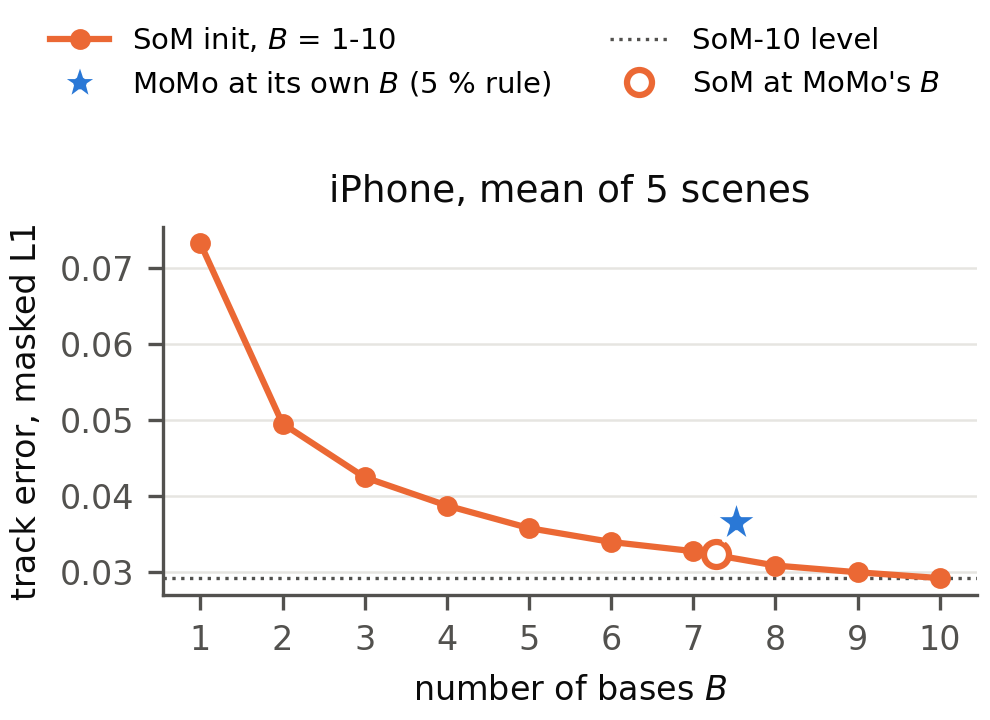
\includegraphics[width=\linewidth]{img/track_error_iphone_avg.png}
  \caption{\claudetag\ \claudeadd{Track error of the initialization (masked $\ell_1$ distance to the 3D tracks, before photometric
    training) against the number of bases, averaged over the five DyCheck (iPhone) scenes: SoM~\cite{wang2025shape} with
    $B = 1$--$10$ bases (curve), MoMo with the number of bases its $\tau = 0.05$ cutoff chooses (star) and SoM with that same number
    (circle); dotted line: SoM-10. Lower is better. Seed 42.}}
  \label{fig:track-avg}
\end{figure}
